\documentclass[tikz,border=12pt]{standalone}
\usepackage{stix}
\usepackage{ifthen}
\usepackage{tikz}
\usepackage{pgfmath}
\usetikzlibrary{angles}
\usetikzlibrary{quotes}
\usetikzlibrary[shadows]
\usetikzlibrary[decorations.pathmorphing]
\usepackage{tkz-euclide}
\usetkzobj{all}
\pgfmathsetmacro{\cubex}{4.5}
\pgfmathsetmacro{\cubey}{5.3}
\pgfmathsetmacro{\cubez}{4.5}
\usetikzlibrary{arrows, arrows.meta}
\usetikzlibrary{intersections}
\usetikzlibrary{decorations.markings}
\usetikzlibrary{angles}
\usetikzlibrary{quotes}
\usetikzlibrary{calc}
\usetikzlibrary{arrows}
\usetikzlibrary{arrows.meta}
\usetikzlibrary{shapes.geometric}
\usetikzlibrary{patterns}
\usetikzlibrary{shapes}



\definecolor{pink1}{RGB}{227,12,116}
\definecolor{blue1}{RGB}{0,51,255}
\definecolor{red1}{RGB}{210,35,42}
\definecolor{red2}{RGB}{211,109,85}
\definecolor{green1}{RGB}{0,153,0}
\definecolor{yellow1}{RGB}{249,159,52}
\definecolor{yellow2}{RGB}{253,195,130}
\begin{document}
	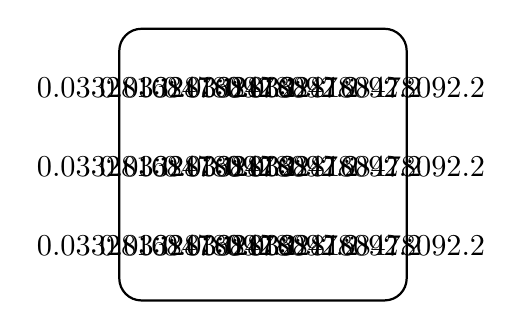
\begin{tikzpicture}
	\pgfgettransformentries{\mya}{\myb}{\myc}{\myd}{\mys}{\myt}
	\pgfmathsetmacro{\preserve}{1/\mya}
	\begin{scope}[>={Stealth[scale=1.2]}, thick, font=\fontsize{11.25}{11.25}\selectfont]
	

\draw [rounded corners=8pt](0.4,0.3) rectangle (4.05,3.75);

\foreach \x in {1,1.8,2.6,3.4}
\foreach \y in {1,2,3}
\node at  (\x,\y)[]{\nagwaPictogram{0.03}{328168478092.2}};
%



\end{scope}
	
	
	\end{tikzpicture}
\end{document}
